\Askhsh{18566_SOLUTION}{1}
\begin{ylh}{1}
    \item [Ύλη από εικόνα]
\end{ylh}
\begin{wrapfigure}[15]{r}{6cm} % Estimated height for the figure
    \centering
    \begin{tikzpicture}[scale=0.7] % Reduced scale slightly to fit better
        % Define points A, B, C for the right-angled triangle
        \tkzDefPoint(0,0){A}
        \tkzDefPoint(4,0){B} % Example length for AB
        \tkzDefPoint(0,3){C} % Example length for AC
        
        % Calculate length of hypotenuse BC (let's call it L_BC)
        \pgfmathsetmacro{\bval}{4} % AB length
        \pgfmathsetmacro{\cval}{3} % AC length
        \pgfmathsetmacro{\LBC}{sqrt(\bval*\bval + \cval*\cval)} % Hypotenuse length

        % Define point Z: on BA extended towards A, such that BZ = BC
        % A=(0,0), B=(b,0), C=(0,c)
        % Z = (b - L_BC, 0)
        \pgfmathsetmacro{\zx}{\bval - \LBC}
        \tkzDefPoint(\zx,0){Z}

        % Define points D, E for the square BΓΔE
        % Vector BΓ is (-b, c)
        % Rotated 90 deg CCW for D, E relative to B, Γ: (-(yc-yb), xc-xb)
        % Vector BC = (-b, c)
        % Rotated vector: (-c, -b)
        % D = C + (-c, -b) = (0,c) + (-c,-b) = (-c, c-b)
        % E = B + (-c, -b) = (b,0) + (-c,-b) = (b-c, -b)
        \pgfmathsetmacro{\dx}{-\cval}
        \pgfmathsetmacro{\dy}{\cval-\bval}
        \pgfmathsetmacro{\ex}{\bval-\cval}
        \pgfmathsetmacro{\ey}{-\bval}
        \tkzDefPoint(\dx,\dy){D}
        \tkzDefPoint(\ex,\ey){E}

        % Define point H for the rhombus BΓHZ
        % BΓHZ is a rhombus, so vector ZH = vector BΓ
        % H = Z + vector BΓ
        % Z = (\bval-\LBC, 0)
        % Vector BΓ = (-\bval, \cval)
        % H_x = (\bval-\LBC) - \bval = -\LBC
        % H_y = 0 + \cval = \cval
        % So H = (-\LBC, \cval)
        \pgfmathsetmacro{\hx}{-\LBC}
        \tkzDefPoint(\hx,\cval){H}

        % Draw the triangle ABΓ
        \tkzDrawSegments(A,B A,C B,C)
        \tkzMarkRightAngle(C,A,B)
        
        % Draw the square BΓΔE
        \tkzDrawSegments(B,C C,D D,E E,B)
        
        % Draw the rhombus BΓHZ
        \tkzDrawSegments(B,C C,H H,Z Z,B)

        % Draw points
        \tkzDrawPoints(A,B,C,D,E,Z,H)

        % Label points
        \tkzLabelPoint[below left](A){A}
        \tkzLabelPoint[below](B){B}
        \tkzLabelPoint[above left](C){$\Gamma$}
        \tkzLabelPoint[below left](D){$\Delta$}
        \tkzLabelPoint[below right](E){E}
        \tkzLabelPoint[below](Z){Z}
        \tkzLabelPoint[above left](H){H}
    \end{tikzpicture}
\end{wrapfigure}
\noindent \kefalaio{ΛΥΣΗ}

\noindent Έστω το ορθογώνιο τρίγωνο \mbox{ΑΒΓ} με $\hat{A} =90^{\circ}$ και \mbox{ΒΓΔΕ} το τετράγωνο με πλευρά την υποτείνουσα \mbox{ΒΓ} του τριγώνου. Προεκτείνουμε την πλευρά \mbox{ΒΑ} προς το \mbox{Α} και παίρνουμε σημείο \mbox{Ζ} τέτοιο ώστε \mbox{ΒΖ} = \mbox{ΒΓ}. Οι παράλληλες από το \mbox{Γ} στη \mbox{ΒΖ} και από το \mbox{Ζ} στη \mbox{ΒΓ} τέμνονται στο \mbox{Η}.

\begin{alist}
    \item Το τετράπλευρο \mbox{ΒΓΗΖ} έχει τις απέναντι πλευρές του παράλληλες, οπότε είναι παραλληλόγραμμο. Επιπλέον οι διαδοχικές πλευρές του \mbox{ΒΓ} και \mbox{ΒΖ} είναι ίσες από την κατασκευή, οπότε το \mbox{ΒΓΗΖ} είναι ρόμβος με πλευρά ίση με την υποτείνουσα \mbox{ΒΓ} του ορθογωνίου τριγώνου \mbox{ΑΒΓ}. Άρα η περίμετρος του ρόμβου είναι ίση με $4 \cdot \text{ΒΓ}$. Επίσης το τετράγωνο \mbox{ΒΓΔΕ} έχει πλευρά ίση με την υποτείνουσα \mbox{ΒΓ} του τριγώνου, άρα η περίμετρός του είναι ίση με $4 \cdot \text{ΒΓ}$. Δηλαδή ο ρόμβος και το τετράγωνο έχουν ίσες περιμέτρους.
    \item Για το εμβαδό του τετραγώνου έχουμε ότι $(\text{ΒΓΔΕ}) = \text{ΒΓ}^2$. Ενώ, για το εμβαδό του ρόμβου, αφού ο ρόμβος είναι παραλληλόγραμμο, έχουμε: $(\text{ΒΓΗΖ}) = \text{ΒΖ} \cdot \text{ΓΑ}$ με \mbox{ΓΑ} η απόσταση των παραλλήλων πλευρών του \mbox{ΒΖ} και \mbox{ΓΗ}. Συγκρίνοντας τα δύο εμβαδά παρατηρούμε ότι, για το εμβαδό του τετραγώνου το τμήμα \mbox{ΒΓ} πολλαπλασιάζεται με το \mbox{ΒΓ} και για το εμβαδό του ρόμβου, το \mbox{ΒΓ} πολλαπλασιάζεται με το \mbox{ΑΓ}. Το τμήμα \mbox{ΑΓ} είναι κάθετη πλευρά του ορθογωνίου τριγώνου \mbox{ΑΒΓ} και το τμήμα \mbox{ΒΓ} είναι υποτείνουσα. Όμως η κάθετη πλευρά είναι πάντα μικρότερη της υποτείνουσας, επομένως το εμβαδό του ρόμβου είναι μικρότερο από το εμβαδό του τετραγώνου και δεν γίνεται ποτέ τα δύο σχήματα να είναι ισεμβαδικά. Άρα ο ισχυρισμός 2 είναι σωστός.
\end{alist}